\documentclass[11pt, oneside]{article} 
\usepackage{geometry}
\geometry{letterpaper} 
\usepackage{graphicx}
	
\usepackage{amssymb}
\usepackage{amsmath}
\usepackage{parskip}
\usepackage{color}
\usepackage{hyperref}

\graphicspath{{/Users/telliott/Github/calculus_book/png/}}
% \begin{center} 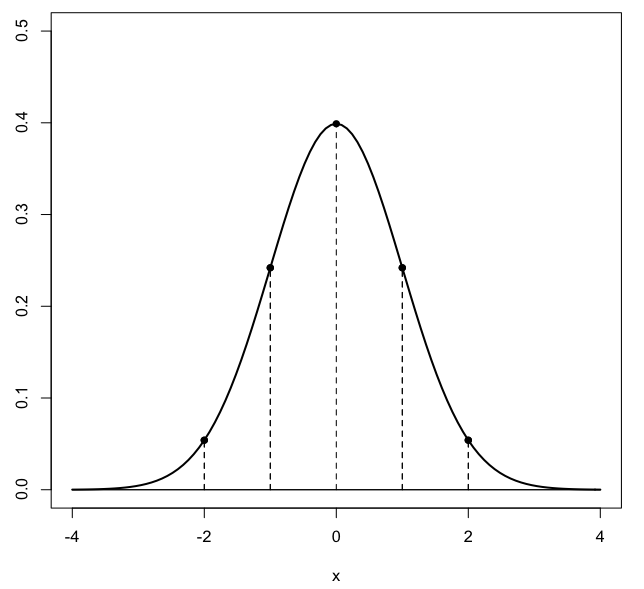
\includegraphics [scale=0.4] {gauss3.png} \end{center}

\title{Arcs of a circle}
\date{}

\begin{document}
\maketitle
\Large
\label{sec:generalized_arc}

We have previously established some central facts about circles including Thales' theorem about the angle intercepting a half-arc of the circle being a right angle.  We will need some of these results later.

We can do more.  We can  generalize the result for all arcs.  

The examples so far contain the diameter in some way. Consider the arc swept out by the angle $\theta$ in this figure (left panel).
\begin{center} 
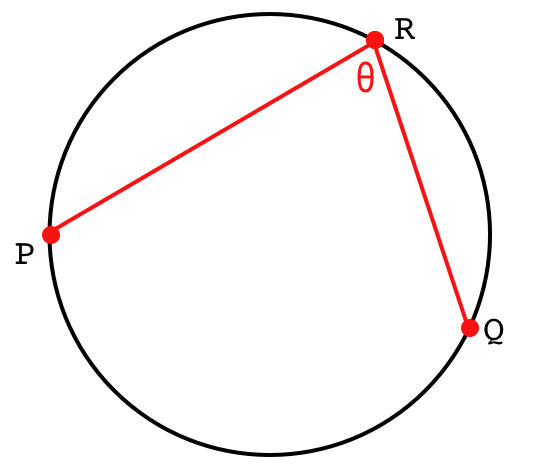
\includegraphics [scale=0.3] {arcs5.png} 
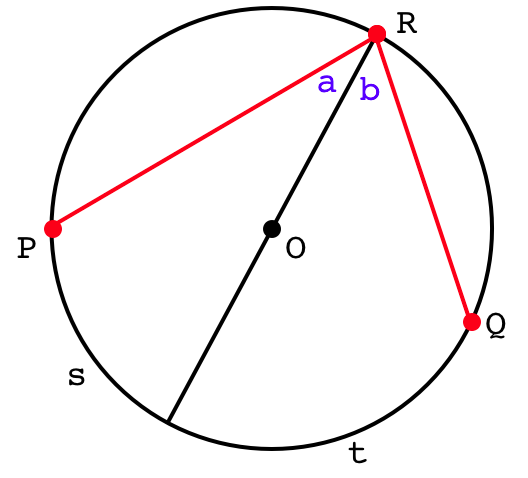
\includegraphics [scale=0.3] {arcs6.png}
\end{center}
We can prove that the measure of the angle $\theta$ is equal to 1/2 the arc swept out between P and Q. For a simple proof, draw the diameter (right panel):
By our previous work:

\[ b = \frac{t}{2}, \ \ \ \ \ \ a = \frac{s}{2} \]
\[ \theta = a + b = \frac{s+t}{2} \]

Thus, we have proved the theorem for the special case where the arc is one-half the circle, for the general case where the diameter is one line segment flanking the angle, and now for another general case where the angle includes the diameter.

However, the theorem is true even if the angle does not include the diameter.  We can establish this by subtraction.
\begin{center} 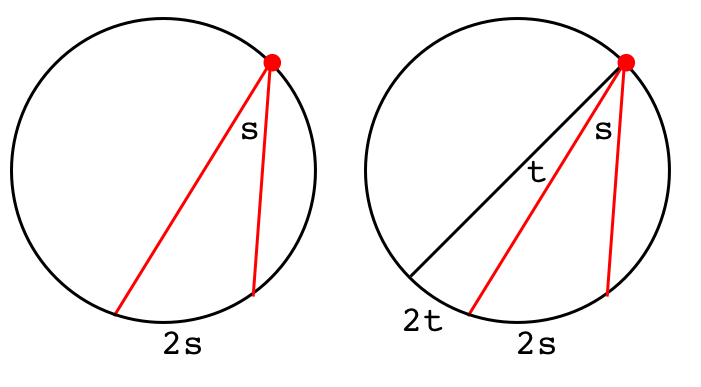
\includegraphics [scale=0.35] {arcs17.png} \end{center}

On the right, draw the diameter.  Notice that we have two arcs which include the diameter:  one with angle $t$ and one with angle $s+t$.  We obtain the generalized arc with angle $s$ by subtracting the result for $t$ from that for $s + t$.

As a corollary, any two angles with vertexes (vertices) on the circle that cut off the same arc are equal.  In the figure below, $s = t$.  Also the triangles (if we draw the bases of the arcs) are similar triangles by AAS.
\begin{center} 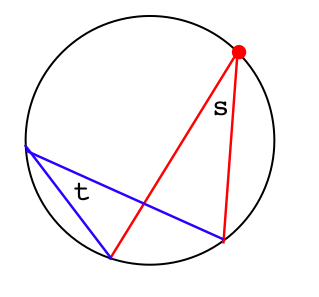
\includegraphics [scale=0.5] {arcs18.png} \end{center}

\subsection*{Intersecting chords}
Given two chords, to prove:

\[ \theta = 1/2 (s + t) \]
$\theta$ is the average of the two arc lengths.

\begin{center} 
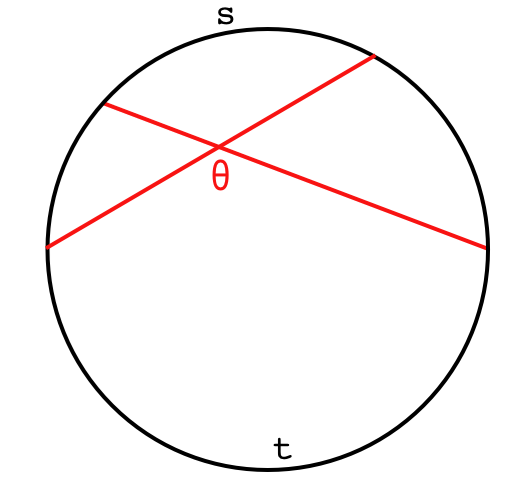
\includegraphics [scale=0.3] {arcs7.png} 
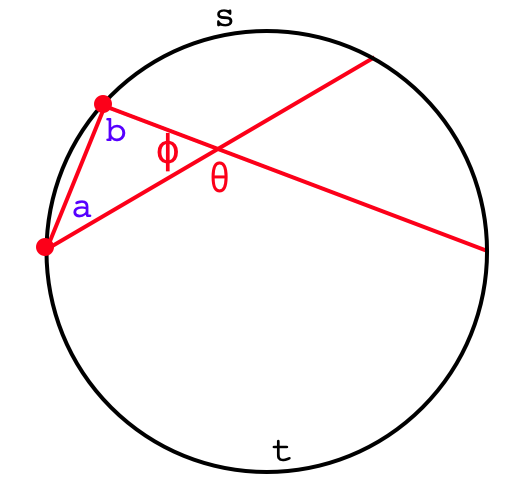
\includegraphics [scale=0.3] {arcs8.png}
\end{center}

Solution:  Draw a triangle (right panel, above).

\[ a = \frac{s}{2}, \ \ \ \ \ \ b = \frac{t}{2} \]
\[ a + b = \theta = \frac{s+t}{2} \]

\subsection*{Tangent and secant}

Rather than having all three points on the circle, one point is now outside. We have the same arc swept out by the endpoints ($t$), but the included angle is now smaller, and there is a new small piece of arc length $s$.

\begin{center} 
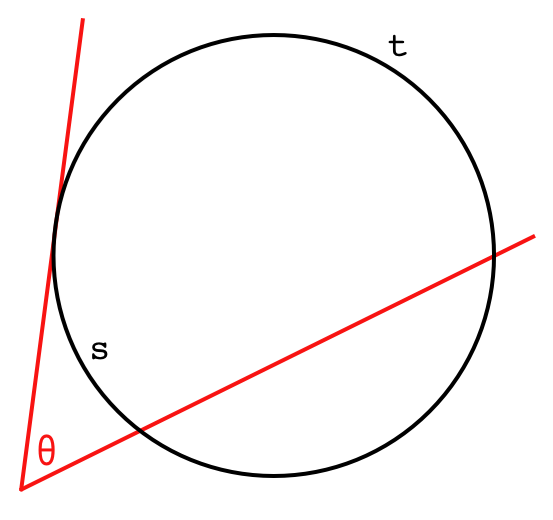
\includegraphics [scale=0.3] {arcs9.png} 
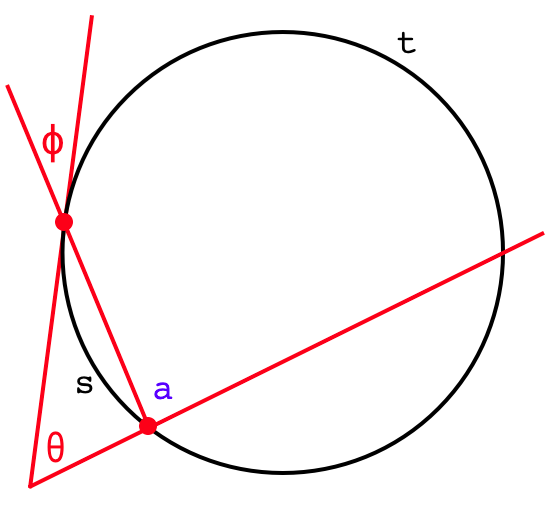
\includegraphics [scale=0.3] {arcs10.png}
\end{center}

To prove:

\[ \theta = \frac{t-s}{2} \]

Solution:
Draw the triangle.  By our previous work (and supplementary angles):

\[ \phi = \frac{s}{2}, \ \ \ \ \ \ a = \frac{t}{2} \]

by supplementary angles:

\[ \theta + \phi = a \]
\[ \theta = \frac{t}{2} - \frac{s}{2} = \frac{t-s}{2} \]

\subsection*{Chord segments}

Finally, there is a simple algebraic relationship between chord segments. Draw two chords of the circle and label the lengths of the segments as shown (note: $s$ and $t$ do not refer to arcs any more).

\begin{center} 
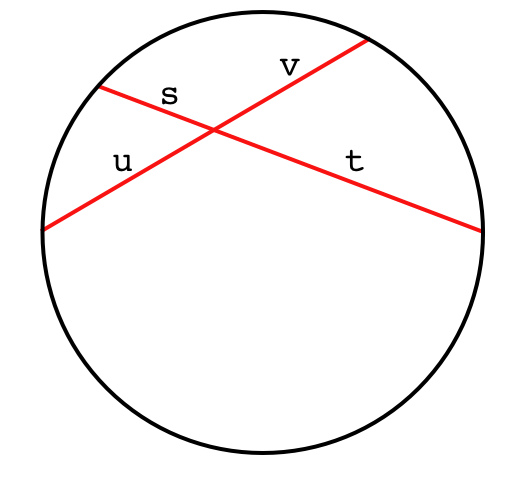
\includegraphics [scale=0.3] {arcs15.png} 
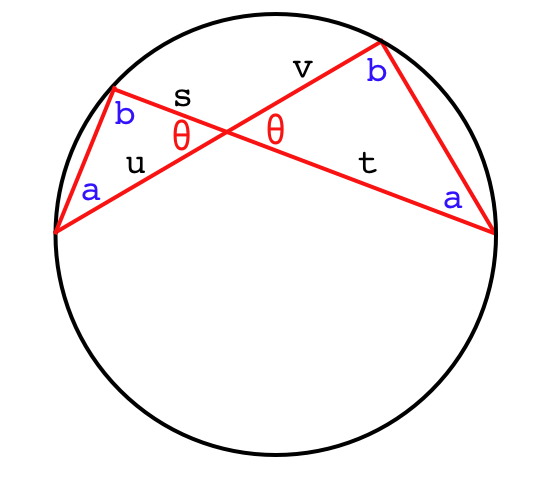
\includegraphics [scale=0.3] {arcs16.png}
\end{center}
Draw the two triangles.
Notice that the two angles labeled $a$ are equal because they sweep out the same arc of the circle, and similarly for the two angles labeled $b$. By similar triangles, then:

\[ s/u = v/t \]
\[ st = uv \]


\end{document}